% !TEX root = ../eval.tex

\section{Results}%
\label{sec:results}


\subsection{Pre-post comparison}%
\label{sub:pre_post}

Notes:
\begin{itemize}
    \item Assumption: there are no confounding effects (either time-varying,
        individual varying, or individual-time varying), so treatment
        assignment is as good as random.

    \item With controls, we assume that there are no confounding variables
        other than the ones we control for.
\end{itemize}

\begin{figure}[htpb]
    \centering
    \caption{Naive pre-post results}%
    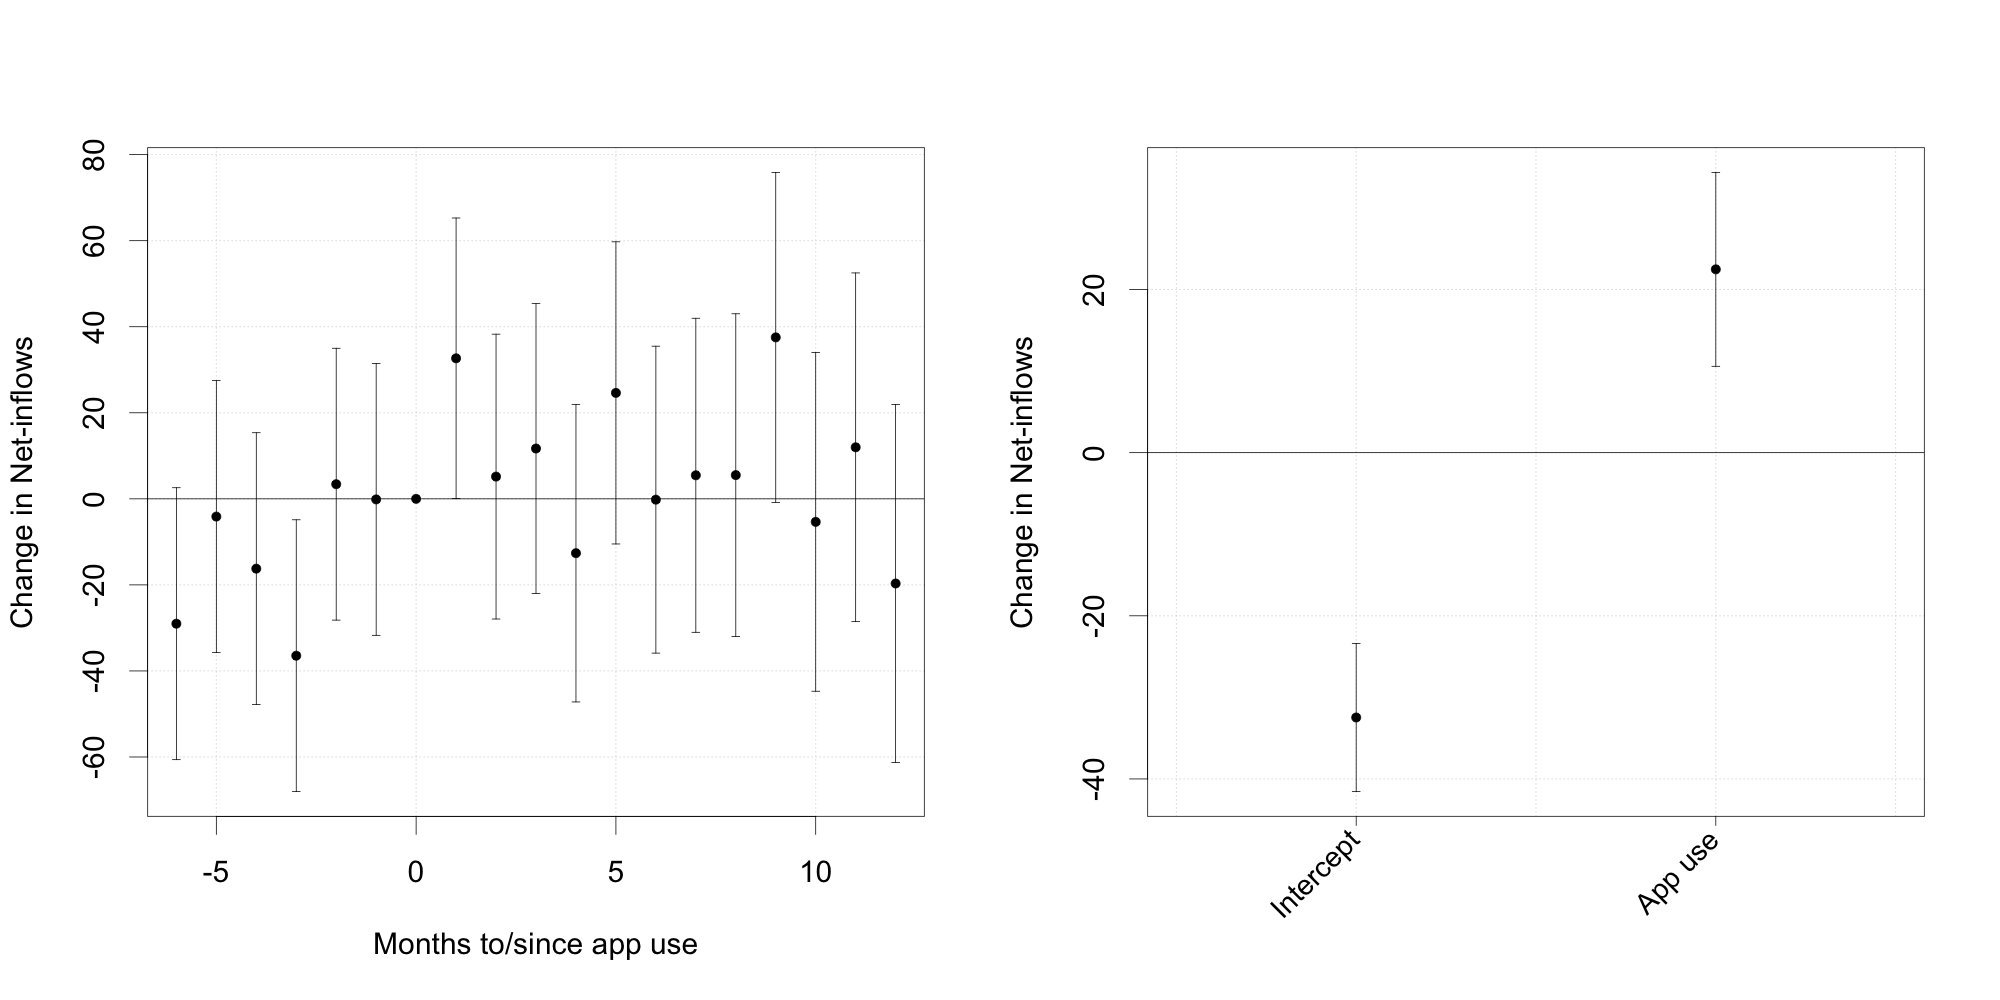
\includegraphics[width=\linewidth]{\figdir/reg_naive_pre_post.png}
    \label{fig:reg_naive_pre_post}
    \fignote{\textwidth}{Notes: ...}
\end{figure}

\begin{figure}[htpb]
    \centering
    \caption{Pre-post with controls}%
    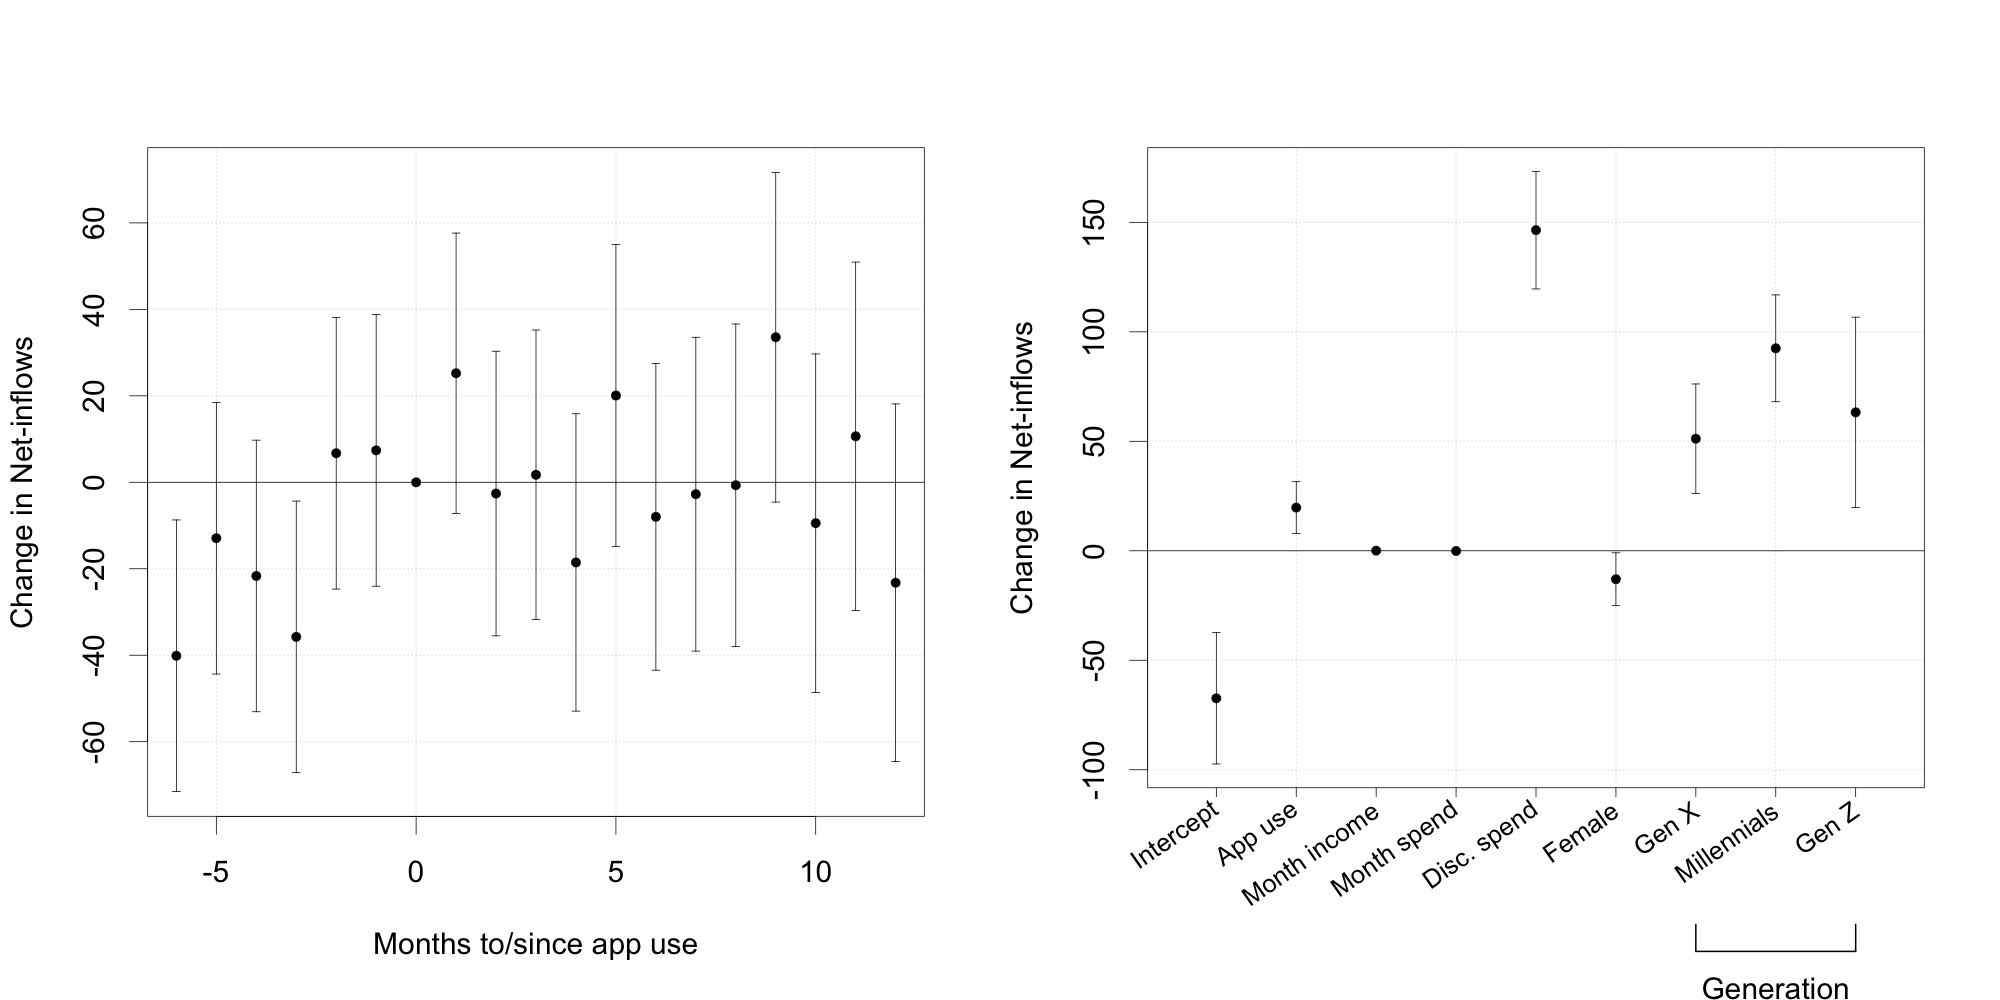
\includegraphics[width=\linewidth]{\figdir/reg_controls.png}
    \label{fig:reg_controls}
    \fignote{\textwidth}{Notes: ...}
\end{figure}


\subsection{Static and dynamic TWFE}%
\label{sub:static_twfe}

Static:
\begin{equation}
    y_{it} = \alpha_i + \lambda_t + \beta T_{it} + \gamma X_{it} + \epsilon_{it}
\end{equation}

Dynamic:
\begin{equation}
    y_{it} = \alpha_i + \lambda_t + \sum^{5}_{s=-6} \beta_s T_{its} + \gamma X_{it} + \epsilon_{it}
\end{equation}

\begin{itemize}

    \item Comparison: pre vs post signup within each individual.

    \item Assumption: there are no time-varying unobserved effects that affect
        both y and T.

    \item Discussion: there is something that made the individual sign up in
        the first place, and it might well be an individual level shock that we
        don't observe (unexpected large expense, loss of job, etc.)

    \item See \citet{imai2021use} for problems with twfe

    \item See \citet{sun2021estimating} for problems with that and compare to
        their approach as implemented in fixest.

\end{itemize}

\begin{figure}[htpb]
    \centering
    \caption{TWFE}%
    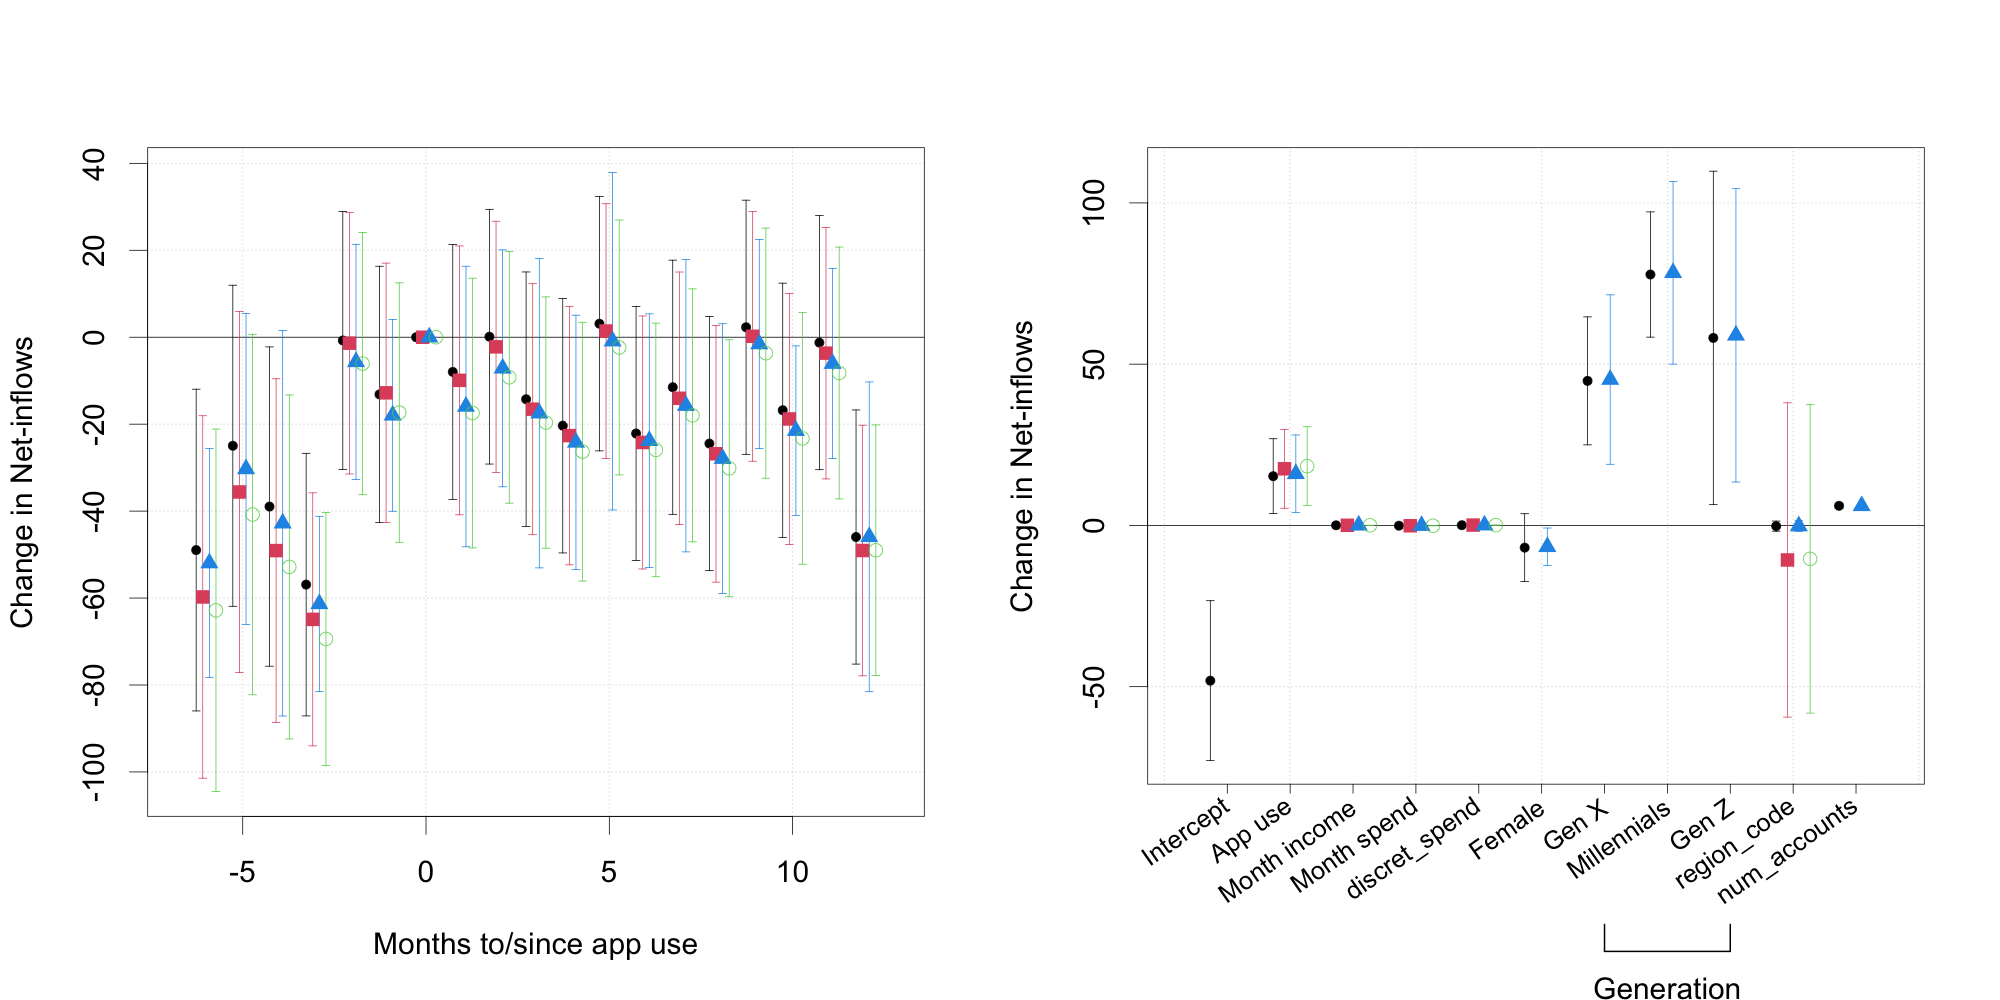
\includegraphics[width=\linewidth]{\figdir/reg_twfe.png}
    \label{fig:reg_twfe}
    \fignote{\textwidth}{Notes: ...}
\end{figure}


\subsection{Dynamic TWFE}%
\label{sub:dynamic_twfe}

\subsection{Matching}%
\label{sub:alternative_matching_method}

\subsection{Post treatment periods as control}%
\label{sub:post_treatment_periods_as_control}

\subsection{Synthetic controls}%
\label{sub:synthetic_controls}

See \citet{abadie2021penalized} for how to use synthetic controls for disaggregated data.


\subsection{Model comparisons}%
\label{sub:model_comparisons}

\begin{figure}[htpb]
    \centering
    \caption{Comparison}%
    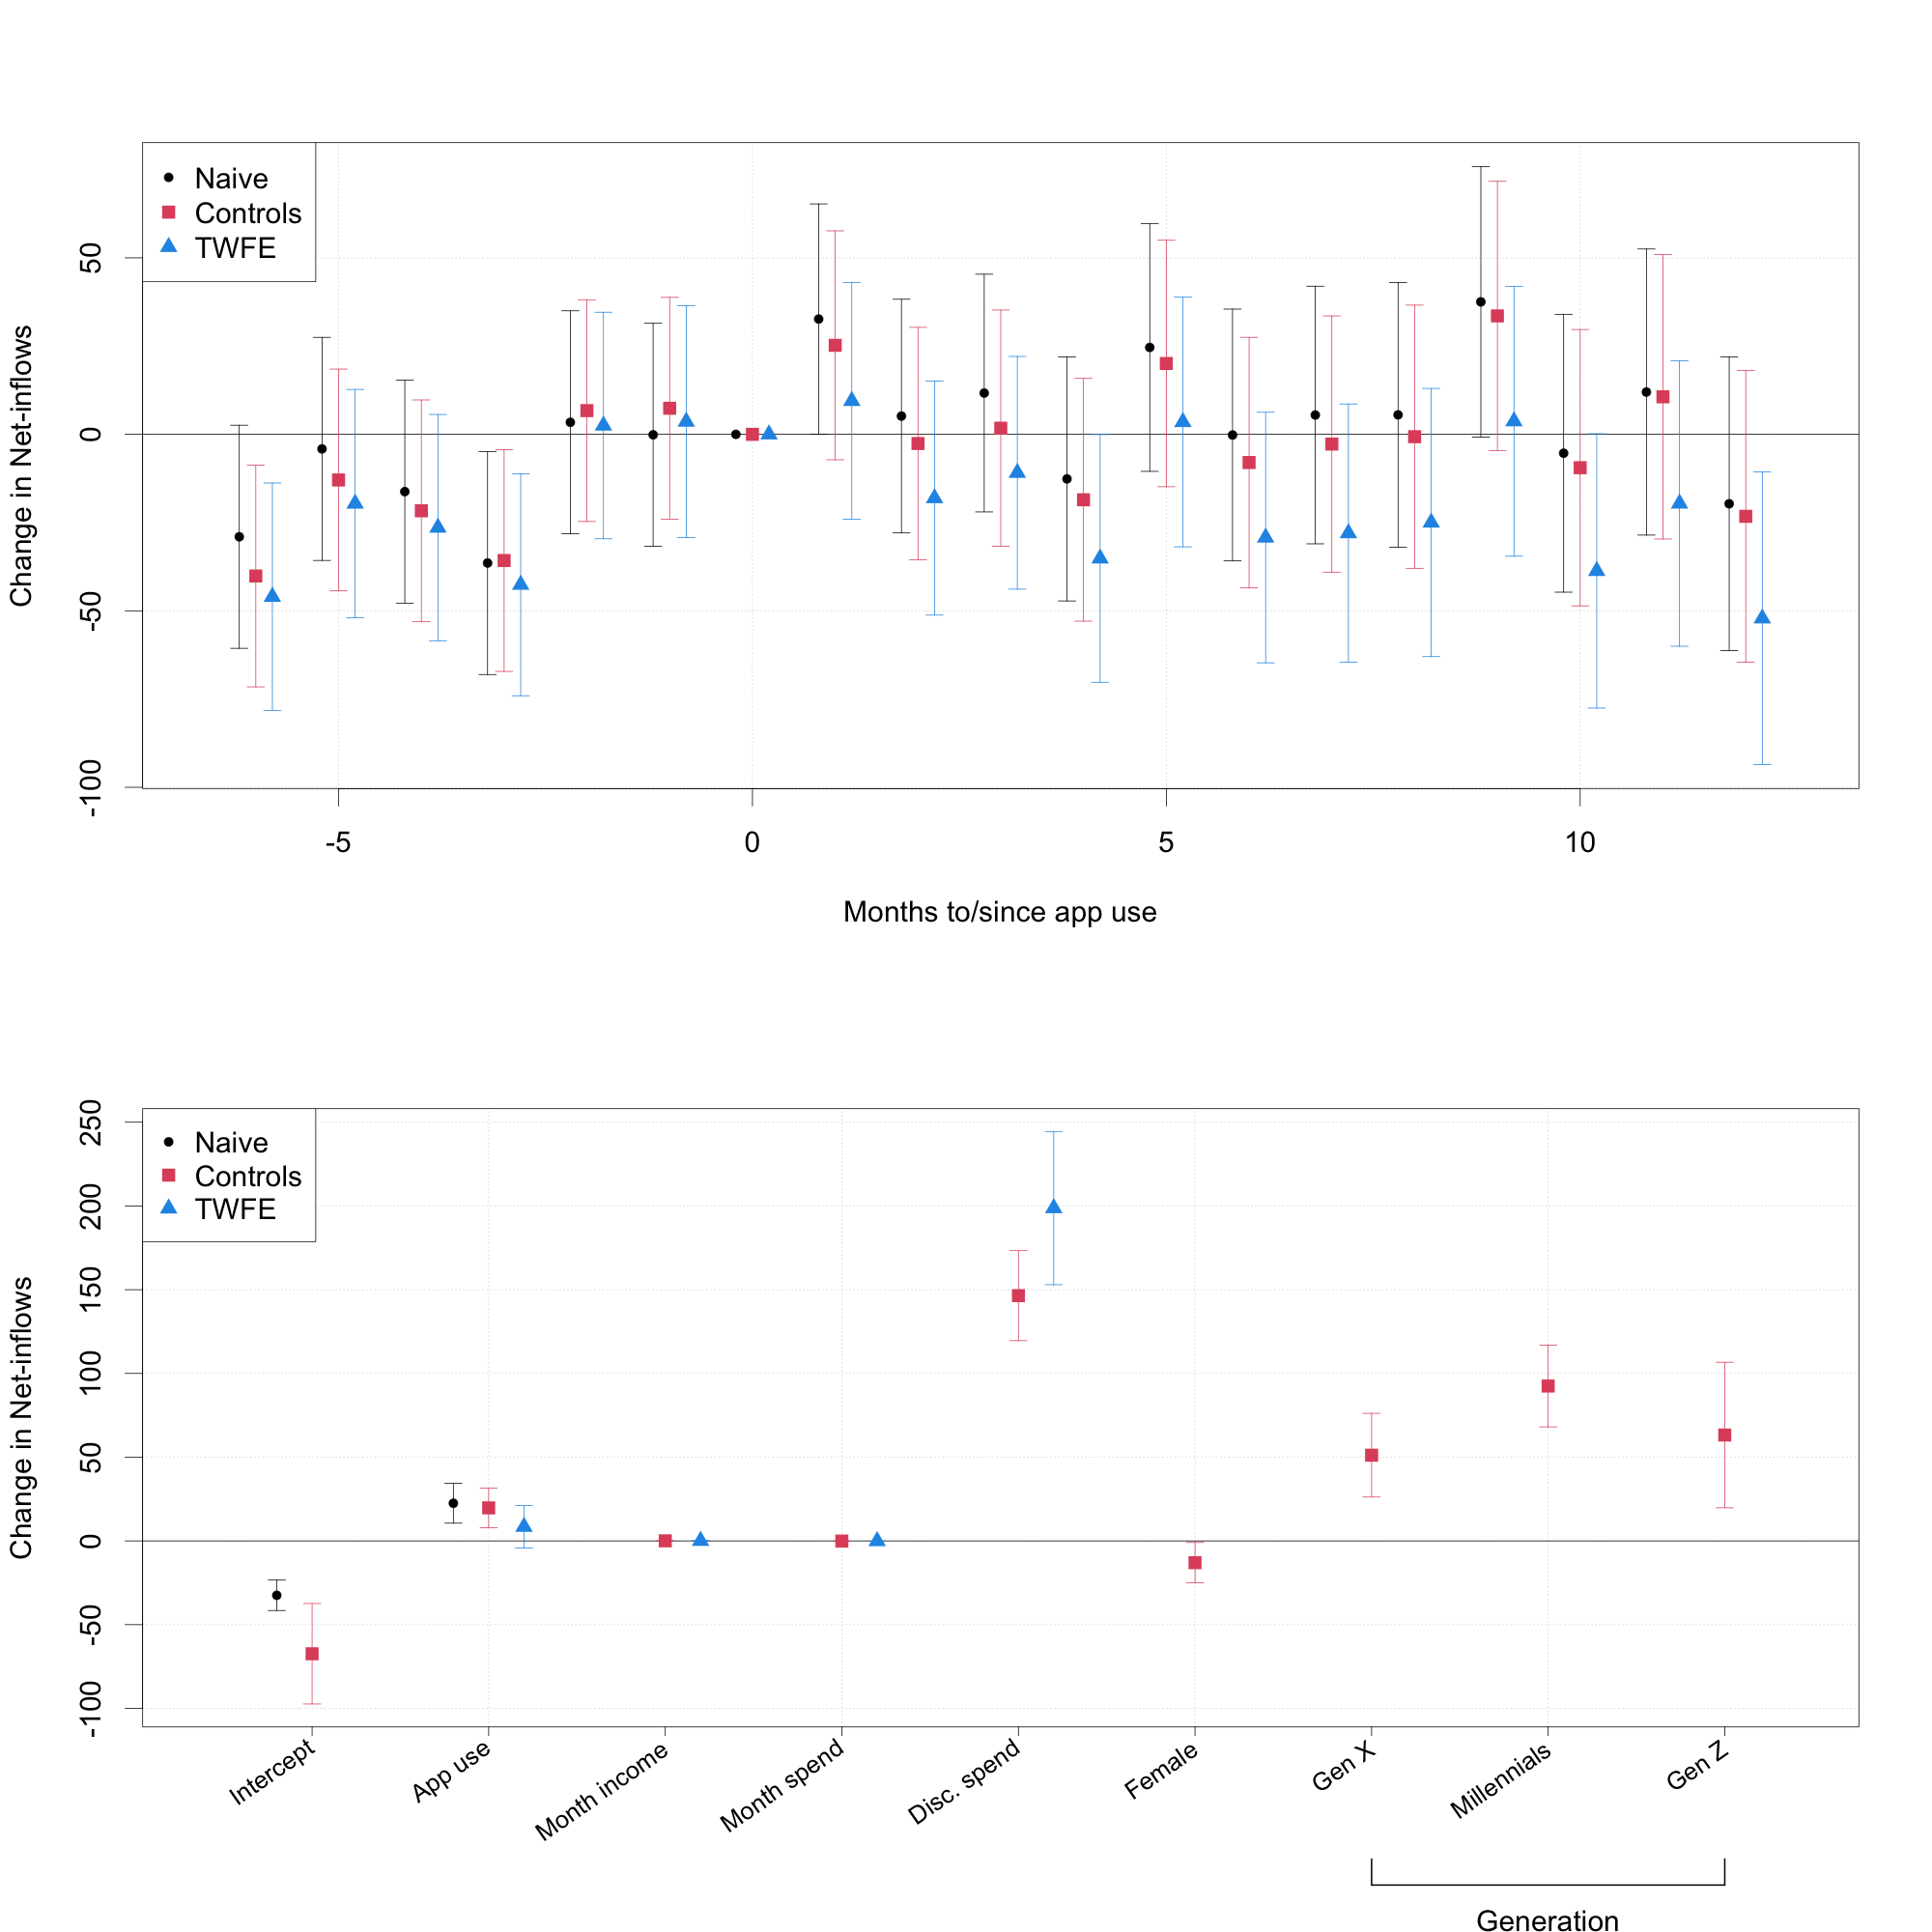
\includegraphics[width=\linewidth]{\figdir/reg_comparison.png}
    \label{fig:reg_comparison}
    \fignote{\textwidth}{Notes: ...}
\end{figure}



\begin{table}[htbp]
   \centering
   \tiny
   \begin{threeparttable}[b]
      \caption{\label{tab:reg_compare} Regression results}
      \begin{tabular}{lccccc}
         \tabularnewline \midrule \midrule
         Dependent Variable: & \multicolumn{5}{c}{Net-inflows}\\
         Model:                     & (1)                   & (2)                & (3)                & (4)               & (5)\\  
         \midrule
         \emph{Variables}\\
         App use                    & 14.330$^{**}$         & 15.303$^{***}$     & 19.381$^{***}$     & 15.963$^{**}$     & 20.207$^{***}$\\   
                                    & [2.650; 26.009]       & [3.686; 26.919]    & [7.110; 31.652]    & [1.881; 30.045]   & [7.940; 32.473]\\   
         Month income               &                       & 0.053$^{***}$      & 0.060$^{***}$      & 0.053$^{***}$     & 0.058$^{***}$\\   
                                    &                       & [0.049; 0.058]     & [0.045; 0.075]     & [0.045; 0.060]    & [0.043; 0.073]\\   
         Month spend                &                       & -0.077$^{***}$     & -0.100$^{***}$     & -0.076$^{***}$    & -0.098$^{***}$\\   
                                    &                       & [-0.081; -0.073]   & [-0.109; -0.091]   & [-0.091; -0.061]  & [-0.107; -0.089]\\   
         Disc. spend                &                       & 138.940$^{***}$    & 169.002$^{***}$    & 132.862$^{***}$   & 156.441$^{***}$\\   
                                    &                       & [115.597; 162.282] & [128.874; 209.129] & [90.975; 174.750] & [115.907; 196.976]\\   
         Female                     &                       & -14.521$^{***}$    &                    & -14.247$^{***}$   &   \\   
                                    &                       & [-24.998; -4.044]  &                    & [-21.206; -7.289] &   \\   
         Generation $=$ GenX        &                       & 39.071$^{***}$     &                    & 39.379$^{**}$     &   \\   
                                    &                       & [19.258; 58.885]   &                    & [9.611; 69.148]   &   \\   
         Generation $=$ Millennials &                       & 71.330$^{***}$     &                    & 71.699$^{***}$    &   \\   
                                    &                       & [51.964; 90.697]   &                    & [40.338; 103.060] &   \\   
         Generation $=$ GenZ        &                       & 42.302             &                    & 43.095$^{*}$      &   \\   
                                    &                       & [-9.381; 93.985]   &                    & [-7.002; 93.192]  &   \\   
         Intercept                  & -20.523$^{***}$       & -59.208$^{***}$    &                    &                   &   \\   
                                    & [-30.679; -10.368]    & [-84.179; -34.237] &                    &                   &   \\   
         \midrule
         \emph{Fixed-effects}\\
         User FE                    &                       &                    & Yes                &                   & Yes\\  
         Month FE                   &                       &                    &                    & Yes               & Yes\\  
         \midrule
         \emph{Fit statistics}\\
         Observations               & 184,847               & 184,847            & 184,847            & 184,847           & 184,847\\  
         R$^2$                      & $3.13\times 10^{-5}$  & 0.01132            & 0.10137            & 0.01203           & 0.10203\\  
         Within R$^2$               &                       &                    & 0.00905            & 0.01117           & 0.00885\\  
         \midrule \midrule
         \multicolumn{6}{l}{\emph{Signif. Codes: ***: 0.01, **: 0.05, *: 0.1}}\\
      \end{tabular}
   \end{threeparttable}
\end{table}





\subsection{Alternative window lengths}%
\label{sub:alternative_window_lengths}

\subsection{Subgroups}%
\label{sub:subgroups}

To analyse which groups benefit most from adopting Money Dashboard, we split
our sample by gender, generation, income quartiles, and pre-adoption savings
behaviour.

We define generations as follows: boomers were born between 1946 and 1964, Gen
X between 1965 and 1980, Millennials between 1981 and 1996, and Gen Z after
1997.\footnote{Based on age ranges provides by
    \href{https://www.beresfordresearch.com/age-range-by-generation/}{Beresford
Research}.}

Subgroup analysis: same Fig an Tab as in main analysis, but with line for each
subgroup. One figure for each of: gender, generations, income terciles,
per-adoption average savings tercile (inspired by \citet{carlin2017fintech},
see Fig 5 and Table 4).

See also section 6 in \citet{gargano2021goal}

